\newpage
%\renewcommand{\baselinestretch}{1.}
\begin{center}
\LARGE \sf
\end{center}
\large
\sf
\noindent
{\em \Large Examples for linear fits}\\[3mm]
Attention: Linear means that 
$y$ depends linearly on the fitparameters $a_i$.
\begin{figure}[h]
\unitlength1cm
  \begin{picture}(8,20.)
    \put(-3.,-2.){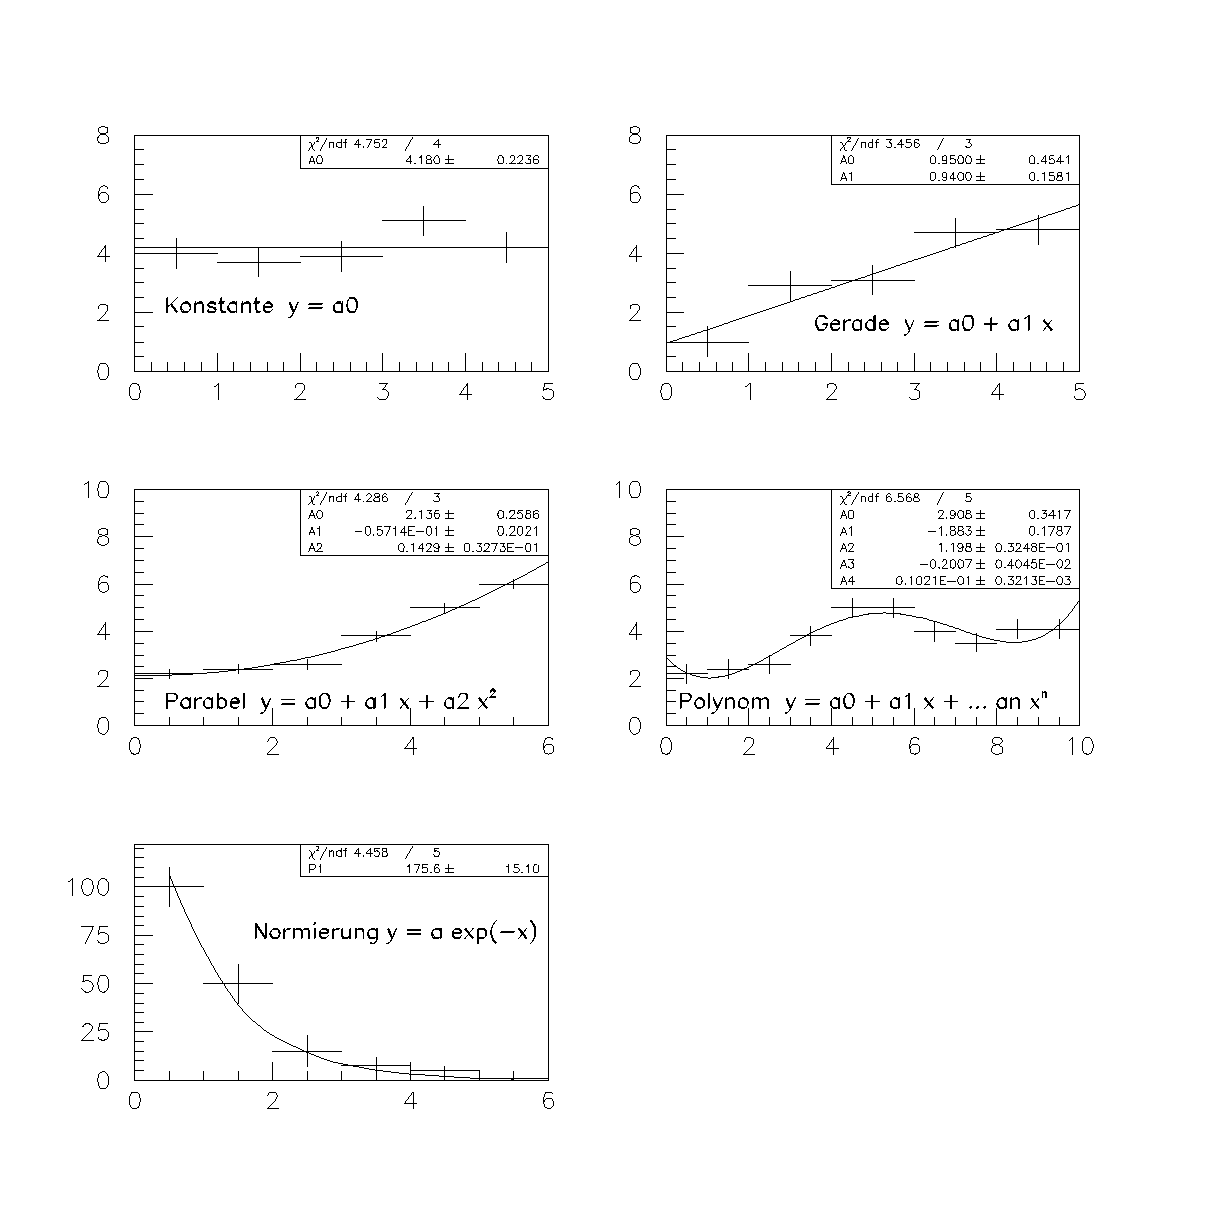
\epsfig{file=eps/linfits.eps,width=22.cm}}
\end{picture}
\end{figure}
